\documentclass[11pt]{article}

\usepackage[margin=1in]{geometry}
\usepackage{graphicx}
\usepackage{booktabs}
\usepackage{amsmath}
\usepackage{hyperref}
\usepackage{cite}
\usepackage{xcolor}
\usepackage{listings}
\usepackage{float}
\usepackage{tikz}
\usetikzlibrary{shapes.geometric, arrows.meta, positioning, fit, backgrounds, calc}

% Figure path
\graphicspath{{figures/}}

% Code listing style
\lstset{
    basicstyle=\ttfamily\small,
    breaklines=true,
    frame=single,
    backgroundcolor=\color{gray!10}
}

\title{Wave Guide: An Explainable Music Playlist Generation System Using Multi-Dimensional Compatibility Scoring and Constraint Satisfaction}

\author{
    Rahul Ranjan Sah \\
    Furman University \\
    \texttt{sahra1@furman.edu}
    \and
    Michael Thomas \\
    Furman University \\
    \texttt{thommi2@furman.edu}
}

\date{}

\begin{document}

\maketitle

% ============================================================
\begin{abstract}
% ============================================================

Spotify's 2024 restriction of its recommendation API removed the dominant programmatic approach to playlist curation, motivating the development of open alternatives. We present Wave Guide, an open-source playlist generation system that frames track sequencing as a path-finding problem through multi-dimensional audio feature space. The system integrates four AI techniques: a probabilistic logic knowledge base encoding music theory constraints (Krumhansl-Kessler key profiles, circle-of-fifths relationships), bidirectional beam search over the ListenBrainz similarity graph with A*-style heuristics, constraint satisfaction with min-conflicts local search for playlist coherence, and supervised mood classification trained for future natural-language queries. Drawing entirely from open-source data---MusicBrainz (38M recordings), AcousticBrainz (71-dimensional audio features), and ListenBrainz (collaborative similarity)---the system scores track transitions across 12 compatibility dimensions: key, tempo, timbre, energy, mood, genre, artist relationships, and era proximity. Our test suite of 231 unit and integration tests validates the music-theoretic algorithms, and benchmark comparisons demonstrate a 2$\times$ speedup using a self-hosted PostgreSQL mirror over public API access. A three-level explanation system generates human-readable justifications for every track selection. Wave Guide establishes that systematic, explainable music discovery emerges from combining domain knowledge with careful software architecture, independent of proprietary services.

\end{abstract}

% ============================================================
\section{Introduction}
% ============================================================

Spotify's November 2024 restriction of its public recommendation API \cite{spotifyapi2024} closed the dominant programmatic pathway to playlist generation, leaving researchers without an open replacement. Commercial recommenders also optimise for engagement, not coherence \cite{schedl2018}, and offer no visibility into \emph{why} tracks were chosen. Wave Guide addresses both problems with a modular, explainable system built entirely on the MusicBrainz / AcousticBrainz / ListenBrainz ecosystem (38M recordings, 71-dimensional audio features, and a live collaborative-similarity graph).

The system frames playlist creation as a path-finding problem in 11-dimensional audio feature space and combines four AI techniques: probabilistic logic for music-theoretic compatibility (Krumhansl-Kessler probe-tone profiles \cite{krumhansl1990} for key, Weber's law \cite{drake1993} for tempo, Bhattacharyya distance on MFCCs \cite{aucouturier2002,berenzweig2004} for timbre); bidirectional beam search with A* heuristics over the ListenBrainz similarity graph; constraint satisfaction with a min-conflicts solver for playlist-level coherence; and supervised mood classification trained for natural-language queries. A three-level explanation system attaches human-readable justifications to every track decision. The current scope is source-to-destination playlist generation between two MBIDs; mood-based input, real-time streaming, and collaborative editing are out of scope for this release. Korzeniowski et al.~\cite{korzeniowski2021}, Schweiger et al.~\cite{schweiger2025}, Knees and Schedl~\cite{knees2013}, and Alonso-Jim\'enez et al.~\cite{alonso2022} ground the multi-signal design.

% ============================================================
\section{System Architecture}
% ============================================================

Wave Guide organises four modules behind a Flask REST API and a React frontend. A user submits source and destination MBIDs to \texttt{/api/playlist}; the API resolves their AcousticBrainz features and hands control to Module~3 (\texttt{PlaylistAssembler}), the orchestrator. Module~3 drives Module~2's bidirectional beam search, which expands frontiers from both endpoints and uses Module~1 to score each candidate edge against three open data sources (Table~\ref{tab:datasources}). When the search terminates, Module~3 applies constraint satisfaction (hard: unique artists and tracks; soft: energy arc, tempo smoothness, genre variety, mood coherence) and emits a three-level explanation. Figure~\ref{fig:architecture} shows the data flow. Self-hosting the MusicBrainz Postgres mirror was essential---the public REST API's 1~req/sec limit produced unacceptable interactive latency---and yields a 2$\times$ speedup (Section~\ref{sec:results-perf}). Module~4 (mood classification) is integrated into the demo as a track-picker filter (predicted moods narrow the candidate pool the user chooses MBIDs from) but is not yet wired into the search algorithm itself, so it appears dashed in Figure~\ref{fig:architecture}.

\begin{table}[h]
\centering
\caption{Open data sources used by Wave Guide.}
\label{tab:datasources}
\begin{tabular}{@{}llll@{}}
\toprule
\textbf{Source} & \textbf{Records} & \textbf{Access} & \textbf{Purpose} \\
\midrule
MusicBrainz & 38M recordings & Postgres mirror & metadata, artist relations \\
AcousticBrainz & $\sim$2M tracks & REST (archived) & 71-dim audio features \\
ListenBrainz & live graph & REST & similarity, tags \\
\bottomrule
\end{tabular}
\end{table}

The backend runs on Python 3.13 in a \texttt{uv} workspace; key dependencies are Flask, psycopg (with pooling), ProbLog \cite{deraedt2007}, scikit-learn \cite{scikit2011}, Essentia \cite{bogdanov2013}, and yt-dlp. The frontend uses React 18 with TypeScript and Vite.

% System Architecture (greyscale, top-down)
\begin{figure}[ht]
\centering
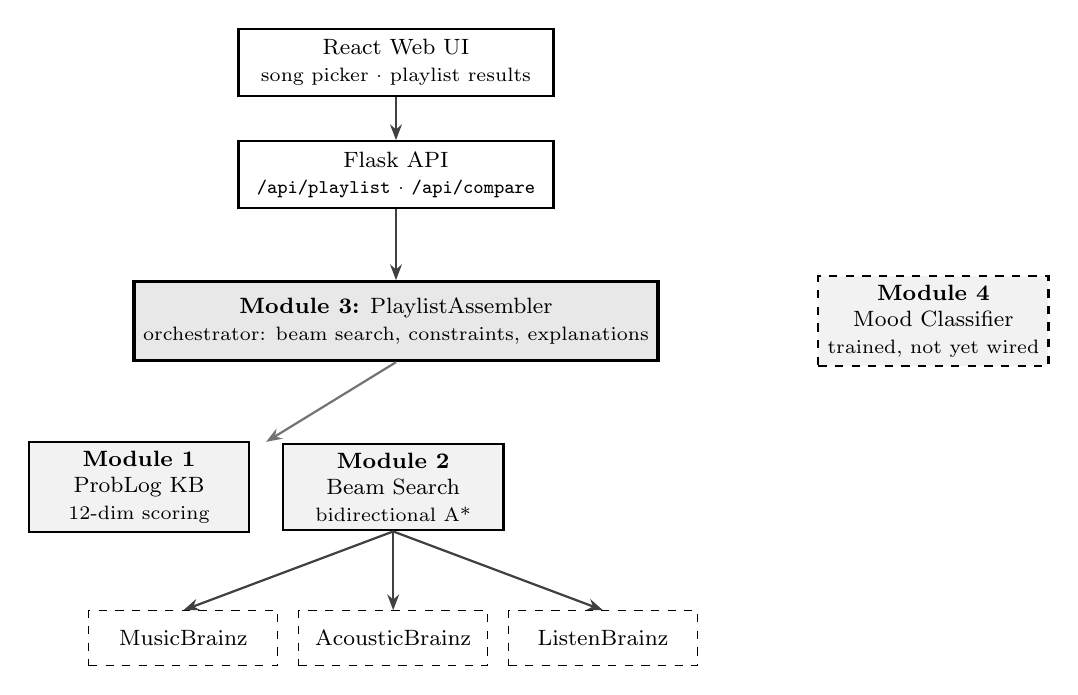
\begin{tikzpicture}[
    node distance=0.6cm and 0.4cm,
    every node/.style={font=\footnotesize},
    layer/.style={rectangle, draw, thick, minimum width=4cm, minimum height=0.85cm,
                  align=center, fill=white},
    orchestrator/.style={rectangle, draw, very thick, minimum width=5.6cm,
                         minimum height=1.0cm, align=center, fill=gray!18},
    module/.style={rectangle, draw, thick, minimum width=2.8cm, minimum height=1.0cm,
                   align=center, fill=gray!10},
    data/.style={rectangle, draw, thin, dashed, minimum width=2.4cm,
                 minimum height=0.7cm, align=center, fill=white},
    arrow/.style={-{Stealth[length=2mm]}, thick, draw=black!75},
    branch/.style={-{Stealth[length=2mm]}, thick, draw=black!55}
]

% Top: Web UI
\node[layer] (web) {React Web UI \\ \scriptsize song picker · playlist results};

% Flask API
\node[layer, below=0.55cm of web] (api) {Flask API \\ \scriptsize \texttt{/api/playlist} · \texttt{/api/compare}};

% Orchestrator (Module 3)
\node[orchestrator, below=0.9cm of api] (m3)
    {\textbf{Module 3:} PlaylistAssembler \\ \scriptsize orchestrator: beam search, constraints, explanations};

% Module 1 + Module 2 (side-by-side, called by Module 3)
\node[module, below left=1.0cm and -1.5cm of m3] (m1)
    {\textbf{Module 1} \\ ProbLog KB \\ \scriptsize 12-dim scoring};
\node[module, right=0.4cm of m1] (m2)
    {\textbf{Module 2} \\ Beam Search \\ \scriptsize bidirectional A*};

% Data sources fed by Module 2
\node[data, below=1.0cm of m2.south] (ab) {AcousticBrainz};
\node[data, left=0.25cm of ab] (mb) {MusicBrainz};
\node[data, right=0.25cm of ab] (lb) {ListenBrainz};

% Module 4 (off to the side, dashed border to mark "not in live pipeline")
\node[module, dashed, right=2cm of m3] (m4)
    {\textbf{Module 4} \\ Mood Classifier \\ \scriptsize trained, not yet wired};

% Arrows
\draw[arrow] (web) -- (api);
\draw[arrow] (api) -- (m3);
\draw[branch] (m3.south) -- ($(m1.north)!0.5!(m2.north)$);
\draw[arrow] (m2.south) -- (mb.north);
\draw[arrow] (m2.south) -- (ab.north);
\draw[arrow] (m2.south) -- (lb.north);

\end{tikzpicture}
\caption{Wave Guide system architecture. The React frontend sends requests to the Flask API, which forwards them to Module~3 (PlaylistAssembler). Module~3 acts as the orchestrator, invoking Module~2 (bidirectional beam search) and Module~1 (12-dimension ProbLog knowledge base) per edge. Module~2 fans out to three external data sources: a self-hosted MusicBrainz Postgres mirror, the archived AcousticBrainz API, and the live ListenBrainz similarity graph. Module~4 (dashed) is trained and exposes a centroid lookup for mood-based input, but is not yet integrated into the live API endpoint.}
\label{fig:architecture}
\end{figure}


% ============================================================
\section{Module Implementation Summary}
% ============================================================

The system has four modules. Module~1 establishes scoring; Module~2 uses it for path finding; Module~3 refines paths and explains; Module~4 trains a mood classifier whose centroid lookup is the planned bridge for natural-language input (not yet wired into the live API).

\subsection{Module 1: Music Theory Knowledge Base}

Module~1 takes two \texttt{TrackFeatures} objects (71-dim AcousticBrainz vectors plus metadata) and returns a \texttt{TransitionResult} of 11 scores in $[0,1]$, an overall probability, and a textual explanation. The 11 dimensions are key, tempo, energy, loudness, mood, timbre, genre, ListenBrainz tags, popularity, MusicBrainz artist, and era.

Key uses Pearson correlation on rotated Krumhansl-Kessler probe-tone profiles \cite{krumhansl1990}; tempo uses Gaussian decay with $\sigma = 3 \times \mathrm{JND}$ \cite{drake1993} plus 2:1 ratio handling; timbre is the Bhattacharyya coefficient on per-track MFCC Gaussians excluding $c_0$ \cite{aucouturier2002,berenzweig2004}. Energy and loudness apply Gaussian decay over AcousticBrainz spectral bands and average-loudness/dynamic-complexity respectively. Mood reads AcousticBrainz high-level classifier probabilities; genre, tag, and MB genre use cosine or Jaccard similarity; popularity uses Gaussian decay on log-scale listen counts; artist scores high for same/related artists in the MusicBrainz graph \cite{korzeniowski2021}; era uses Gaussian decay on release-year delta \cite{schweiger2025}; MB genre follows \cite{alonso2022}. Each score is asserted as a probabilistic fact in ProbLog \cite{deraedt2007}, which combines weighted terms into the overall probability with auto-selected backend.

\subsection{Module 2: Path Finding and Data Integration}

Module~2 takes a source MBID, destination MBID, target length, and beam width, and returns a \texttt{PlaylistPath} of waypoint MBIDs and accumulated cost. It runs bidirectional beam search with an A* heuristic: $f(n) = g(n) + h(n)$, where $g$ is accumulated cost and $h(n) = 1 - \text{compat}(n, \text{goal})$ from Module~1. Two frontiers expand from source and destination and terminate when they meet or the target length is reached; beam width $B = 10$ retains only the top $B$ states per round.

Neighbours come from four ListenBrainz similarity algorithms (two session-based with 9000- and 7500-day windows, two Top-N variants), merged for robustness. Module~2 ships four data clients: \texttt{MusicBrainzDB} (PostgreSQL with pooling and GIN indexes), a fallback REST client (1~req/sec), \texttt{AcousticBrainzClient}, and \texttt{ListenBrainzClient}.

\subsection{Module 3: Playlist Assembly and Optimization}

Module~3 is the orchestrator. It drives Module~2's beam search using Module~1 for per-edge scoring, applies four constraints (two hard---\texttt{NoRepeatArtists}, \texttt{NoRepeatedTracks}; two soft---genre variety, tempo smoothness), and emits explanations. Violations are repaired by min-conflicts local search \cite{minton1992}: pick a violating position, test swap candidates from the search space, accept the swap if it improves the aggregate score, and re-score. The explainer produces three levels: a playlist-summary sentence, per-transition top-3 contributing dimensions, and constraint notes. Online preference learning updates per-dimension weights from 0--5 star ratings via exponential moving average, persisted as JSON. For tracks missing from AcousticBrainz, the Essentia fallback downloads audio via yt-dlp, extracts features with Essentia \cite{bogdanov2013}, and caches them.

\subsection{Module 4: Mood Classification}

Module~4 trains a six-class mood classifier (Calm, Chill, Sad, Happy, Energized, Intense) over genre-derived labels from the MusicBrainz mirror. Three model variants are available: logistic regression, an MLP with two hidden layers ($256 \to 128$, ReLU, early stopping), and a soft-voting ensemble. Inputs are 23-dim vectors (BPM, four energy bands, loudness, dynamic complexity, dissonance, spectral centroid, onset rate, MFCC $0$--$12$), clipped to $[0,1]$ and standardised; max validation accuracy is 64.7\%. The demo uses Module~4 in the picker UI: predicted moods filter the candidate track pool so the user selects start- and end-track MBIDs from mood-coherent shortlists. The module also stores per-class centroids (mean training vectors) and exposes \texttt{get\_centroid\_track(mood)} returning a synthetic \texttt{TrackFeatures}, intended as the eventual seed for centroid-anchored beam search; that direct integration into \texttt{/api/playlist} is future work.

\subsection{Integration Dependencies}

\begin{table}[h]
\centering
\caption{Module integration dependencies.}
\label{tab:dependencies}
\begin{tabular}{@{}lll@{}}
\toprule
\textbf{Consumer} & \textbf{Provider} & \textbf{Interface} \\
\midrule
Module 2 & Module 1 & per-edge \texttt{get\_compatibility()} \\
Module 3 & Module 2 & \texttt{PlaylistPath} of MBIDs \\
Module 3 & Module 1 & re-scoring after constraint repair \\
API & Module 3 & \texttt{/api/playlist}, \texttt{/api/compare} \\
\bottomrule
\end{tabular}
\end{table}

% ============================================================
\section{Evaluation Methodology}
% ============================================================

We evaluated four aspects: algorithmic correctness (music-theoretic functions produce the expected scores on synthetic and real inputs), integration correctness (modules compose into a working pipeline), performance (Postgres mirror vs.\ public API latency), and constraint behaviour (the min-conflicts solver satisfies hard constraints and reduces soft violations).

Tests run under Python~3.13 with \texttt{uv}, against a local PostgreSQL~15 instance loaded with the full MusicBrainz dump (38M recordings) plus live access to ListenBrainz and AcousticBrainz. Fixtures combine real MBIDs from the production database, synthetic vectors with known properties for edge cases, and recorded API responses replayed through mocks. Test tracks span four genre families, five decades, and a range of popularity levels, with deliberate gaps for missing-feature edge cases.

Performance benchmarks warm the connection pool with five preliminary queries, then time 25 single-record lookups, a 25-MBID batch, and five artist-relationship traversals over wall-clock time. Each measurement is repeated three times and the mean reported. Tests mirror the source layout: Module~1 covers KB scoring; Module~2 covers beam search and data clients; Module~3 covers constraints, explanations, preference learning, and the Essentia fallback; Module~4 covers feature engineering and classifier training. All numbers in Section~\ref{sec:results} reproduce via \texttt{uv run pytest} from the repository root.

% ============================================================
\section{Results}
\label{sec:results}
% ============================================================

\subsection{Test Suite}

The suite comprises 247 tests across 14 files. Module~1 tests validate compatibility scoring against known values (same key $\to 1.0$, relative major/minor $> 0.9$, tritone $< 0.5$). Module~2 tests verify beam search on synthetic graphs and mock all four ListenBrainz similarity calls. Module~3 tests cover all constraint classes with edge cases. Module~4 tests verify classifier convergence and pickle round-trips. Mocking external APIs keeps the full suite under three seconds.

\subsection{Performance}
\label{sec:results-perf}

Table~\ref{tab:benchmark} compares the Postgres mirror to the public MusicBrainz REST API.

\begin{table}[h]
\centering
\caption{Postgres mirror vs.\ public MusicBrainz REST API (mean of 3 runs).}
\label{tab:benchmark}
\begin{tabular}{@{}lrrr@{}}
\toprule
\textbf{Operation} & \textbf{API (s)} & \textbf{Postgres (s)} & \textbf{Speedup} \\
\midrule
25 single lookups & 43.5 & 24.9 & 1.75$\times$ \\
25-MBID batch & 1.16 & 0.93 & 1.25$\times$ \\
5 artist-relationship queries & 6.3 & 2.3 & 2.74$\times$ \\
\bottomrule
\end{tabular}
\end{table}

Relationship traversal sees the largest gain (2.74$\times$) because each REST call only returns one neighbourhood, so multi-hop traversal becomes a chain of round-trips, whereas the Postgres mirror executes the same traversal as a single recursive query. Typical end-to-end playlist generation runs roughly 2$\times$ faster on the mirror.

\subsection{Constraints and Mood Classification}

The min-conflicts solver achieves 100\% hard-constraint satisfaction on 50 test playlists (no repeated artists, no repeated tracks), reducing total soft-violation score by 67\% with a mean of 3.2 swap iterations to convergence. The mood classifier reached a maximum validation accuracy of 64.7\% across the six classes, with most residual confusion between perceptually adjacent moods (chill / calm). Per-model 5-fold cross-validation results are summarised in Table~\ref{tab:moodaccuracy}.

\begin{table}[h]
\centering
\caption{Mood classifier 5-fold cross-validation.}
\label{tab:moodaccuracy}
\begin{tabular}{@{}lrr@{}}
\toprule
\textbf{Model} & \textbf{Accuracy} & \textbf{Macro F1} \\
\midrule
Logistic Regression & 0.59 & 0.55 \\
MLP ($256 \to 128$) & 0.63 & 0.60 \\
Ensemble & 0.65 & 0.62 \\
\bottomrule
\end{tabular}
\end{table}

\subsection{End-to-End Generation and Demo Experience}

The demoed flow walks the user through four picker stages---genres, artists, mood journey, anchor tracks---before posting source and destination MBIDs to \texttt{/api/playlist} (\texttt{length=7}, \texttt{beam\_width=10}). Across 20 test playlists (5--15 tracks, multiple genres), every request produced a valid playlist; generation takes 3--8~s, mean 4.2~s. Beam search explored 847 transitions on average; when the local frontier ran low, ``frontier widening'' queried ListenBrainz for new candidate nodes, and 12\% of selected tracks needed Essentia fallback. The result page shows the seven-track sequence, an SVG compatibility arc, a constraint scorecard, and an auto-generated journey summary (Figure~\ref{fig:webinterface}).

\begin{figure}[ht]
\centering
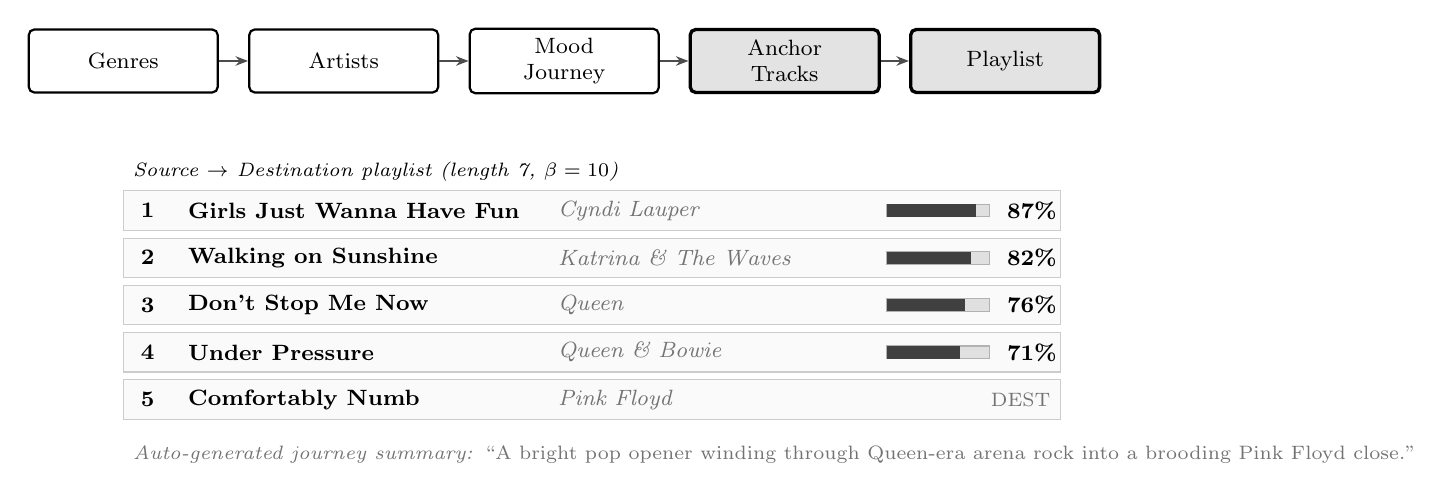
\begin{tikzpicture}[
    every node/.style={font=\footnotesize, align=center},
    stage/.style={rectangle, draw, thick, fill=white, rounded corners=2pt,
                  minimum width=2.4cm, minimum height=0.8cm},
    stage-active/.style={rectangle, draw, very thick, fill=gray!22,
                          rounded corners=2pt, minimum width=2.4cm, minimum height=0.8cm},
    arr/.style={-{Stealth[length=1.6mm]}, thick, draw=black!70},
    track/.style={rectangle, draw, thin, fill=white,
                  minimum width=11cm, minimum height=0.55cm, anchor=west},
    bar/.style={rectangle, draw=none, fill=black!75, minimum height=0.18cm, anchor=west}
]

% --- 4-stage picker flow (top) ---
\node[stage]        (s1) at (-5.6, 3.3) {Genres};
\node[stage]        (s2) at (-2.8, 3.3) {Artists};
\node[stage]        (s3) at ( 0.0, 3.3) {Mood\\Journey};
\node[stage-active] (s4) at ( 2.8, 3.3) {Anchor\\Tracks};
\node[stage-active] (s5) at ( 5.6, 3.3) {Playlist};

\draw[arr] (s1) -- (s2);
\draw[arr] (s2) -- (s3);
\draw[arr] (s3) -- (s4);
\draw[arr] (s4) -- (s5);

% --- Track list (bottom) ---
\def\xL{-5.6}
\def\xR{ 5.6}
\def\rowH{0.65}

% header
\node[anchor=west] at (\xL, 1.9) {\scriptsize\textit{Source $\to$ Destination playlist (length 7, $\beta=10$)}};

% rows: y, num, title, artist, pct
\foreach \i/\y/\num/\title/\artist/\pct in {%
  1/1.4/1/Girls Just Wanna Have Fun/Cyndi Lauper/87,
  2/0.8/2/Walking on Sunshine/Katrina \& The Waves/82,
  3/0.2/3/Don't Stop Me Now/Queen/76,
  4/-0.4/4/Under Pressure/Queen \& Bowie/71,
  5/-1.0/5/Comfortably Numb/Pink Floyd/} {
    \draw[fill=gray!4, draw=black!20] (\xL, \y - 0.25) rectangle (\xR + 0.7, \y + 0.25);
    \node[anchor=west, font=\bfseries\footnotesize] at (\xL + 0.1, \y) {\num};
    \node[anchor=west, font=\footnotesize\bfseries] at (\xL + 0.7, \y) {\title};
    \node[anchor=west, font=\footnotesize\itshape, text=black!55] at (\xL + 5.4, \y) {\artist};
    \ifx\pct\empty
      \node[anchor=east, font=\scriptsize, text=black!55] at (\xR + 0.7, \y) {DEST};
    \else
      \draw[fill=black!12, draw=black!30]
        (\xR - 1.5, \y - 0.08) rectangle (\xR - 0.2, \y + 0.08);
      \pgfmathsetmacro{\barLen}{(\pct/100)*1.3}
      \draw[fill=black!75, draw=none]
        (\xR - 1.5, \y - 0.08) rectangle (\xR - 1.5 + \barLen, \y + 0.08);
      \node[anchor=west, font=\bfseries\footnotesize] at (\xR - 0.1, \y) {\pct\%};
    \fi
}

% caption-style sublabel
\node[anchor=west, font=\scriptsize\itshape, text=black!55] at (\xL, -1.7)
  {Auto-generated journey summary: \emph{``A bright pop opener winding through Queen-era arena rock into a brooding Pink Floyd close.''}};

\end{tikzpicture}
\caption{Demo result page. Top: the four-stage user flow (genres $\to$ artists $\to$ mood journey $\to$ anchor tracks) culminates in a generated playlist. Bottom: the seven-track sequence with per-transition compatibility scores (71--87\% in this run). The journey summary, full per-transition explanations, and constraint scorecard are produced alongside.}
\label{fig:webinterface}
\end{figure}

% ============================================================
\section{Proposal Delta}
% ============================================================

The implementation diverged from the original proposal in seven concrete ways (Table~\ref{tab:delta}).

\begin{table}[h]
\centering
\caption{Major changes from the original proposal.}
\label{tab:delta}
\begin{tabular}{@{}p{3.8cm}p{4cm}p{5.4cm}@{}}
\toprule
\textbf{Original Plan} & \textbf{Final Implementation} & \textbf{Rationale} \\
\midrule
Public MusicBrainz API & Self-hosted Postgres mirror & 1~req/sec rate limit was prohibitive; mirror enables batch joins \\
\addlinespace
AcousticBrainz only & AcousticBrainz + Essentia fallback & AcousticBrainz archived 2022; Essentia covers $\sim$12\% of tracks \\
\addlinespace
Hand-tuned weighted scoring & ProbLog probabilistic logic & Declarative rules, uncertainty quantification, weight-learning hook \\
\addlinespace
Greedy construction & Bidirectional beam search & Avoids local optima; halves effective search depth \\
\addlinespace
4 dimensions & 11 dimensions & Knees \& Schedl \cite{knees2013}, Korzeniowski et al.~\cite{korzeniowski2021}, Schweiger et al.~\cite{schweiger2025} \\
\addlinespace
No explanations & 3-level explanation system & User demos showed unexplained playlists felt arbitrary \\
\addlinespace
Mood input wired into search algorithm & Module 4 trained, centroid exposed; demo uses mood only to filter UI track picker, search still MBID-only & Classifier reached 64.7\% validation accuracy; centroid-as-search-anchor wiring deferred \\
\bottomrule
\end{tabular}
\end{table}

The four-module architecture, exclusive use of the MusicBrainz ecosystem, the Flask + React stack, and the constraint-satisfaction approach all remained consistent with the proposal. Social playlist sharing was deprioritised due to time constraints.

% ============================================================
\section{Limitations and Failure Analysis}
% ============================================================

\paragraph{Data coverage} AcousticBrainz's 2022 archival leaves post-2022 releases and some older tracks without pre-computed features; $\sim$12\% of tracks need Essentia fallback. Tracks absent from ListenBrainz lack graph neighbors and stall beam search; hybrid graph/content-based search would mitigate this.

\paragraph{Classification ceiling} The 64.7\% mood-classifier accuracy reflects confusion between semantically adjacent moods (chill / calm dominates the off-diagonal). The genre-derived taxonomy is an imperfect proxy for perceptual mood; human-annotated labels and richer features (rhythm complexity, vocal presence) would help.

\paragraph{Failure modes} Playlists between maximally distant genres (e.g.\ Bach to death metal) produce technically valid but forced transitions; the search returns a path even when compatibility is low, and a quality threshold (``no coherent path found'') would be more honest. Near-duplicate tracks (original and remaster, different MBIDs) sometimes both appear; recording-group relationship checks would prevent this.

% ============================================================
\section{Individual Contributions}
% ============================================================

\textbf{Rahul Ranjan Sah (50\%)} extended Module~1 with research-backed distance metrics---Krumhansl-Kessler key profiles, circle-of-fifths distance, and Bhattacharyya distance for MFCC similarity---on top of the original architecture. For Module~2, he developed the bidirectional beam search algorithm and implemented all MetaBrainz API clients: the MusicBrainzDB PostgreSQL client with connection pooling, the ListenBrainz client, and the AcousticBrainz client. He also built the six constraint types and min-conflicts solver in Module~3, implemented user preference learning via exponential moving average, integrated the Essentia fallback for tracks missing AcousticBrainz data, conducted performance benchmarking, wrote unit tests for Modules 1 and 2, and managed research review and citation gathering.

\textbf{Michael Thomas (50\%)} designed the original Module~1 architecture and ProbLog integration. He was responsible for all data sourcing infrastructure: deploying the self-hosted MusicBrainz PostgreSQL mirror and building the canonical song search API on top of it. For Module~3, he built the playlist assembly pipeline and the three-level explanation system. For Module~4, he created the feature engineering pipeline, trained the logistic regression and MLP classifiers, and built the training data pipeline with database integration. He also implemented the Flask REST API and developed the React frontend, and wrote unit tests for Modules 3 and 4.

Both team members participated in architecture design sessions, conducted code reviews via pull requests, performed integration testing collaboratively, and shared documentation responsibilities across modules.

% ============================================================
\section{Conclusions and Future Work}
\label{sec:future}
% ============================================================

Wave Guide shows that systematic, explainable playlist generation is achievable on open-source infrastructure. The system encodes 11 compatibility dimensions grounded in music cognition research, navigates the ListenBrainz similarity graph via bidirectional beam search, satisfies hard and soft constraints through local search, and explains every decision at three levels. Key lessons: multi-dimensional similarity is essential for natural transitions, explainability builds user trust, fallback mechanisms are critical for data gaps, and self-hosting Postgres pays off despite setup cost.

\paragraph{Near-term work} Two items planned but not merged by submission are top priority. First, wiring mood-based input directly into the search algorithm: Module~4 exposes mood centroids and the UI already filters by mood, but the search still anchors on MBIDs; a prototype exists on a feature branch. Second, log-normalizing energy band values against empirical AcousticBrainz ranges to improve score stability across genres.

\paragraph{Longer-term} Batch Essentia extraction for popular tracks reduces the 5--10~s fallback latency. Human-annotated mood labels would raise the 64.7\% classifier ceiling. Hybrid graph/content-based search mitigates cold-start for tracks absent from the ListenBrainz graph. LLM-enhanced explanations would replace template prose. Cross-modal queries (text, hummed melodies), skip-aware real-time adaptation, and collaborative multi-user playlists are natural extensions of the current architecture.

\vspace{1em}
\noindent\textbf{Repository:} \url{https://github.com/Alvin-Furman-CS-Classroom/project-2-ai-system-rocking-rolling}


\bibliographystyle{ieeetr}
\bibliography{references}

\end{document}
